\chapter{Introduction}
The topic of Cloud Computing is gaining more and more
attention in the service research community. The main idea is
to make applications available on flexible execution
environments primarily located in the Internet. Several
flavours are known, and three important ones are depicted in
the Figure 1.1 .

\begin{figure}[h]
\begin{center}

\includegraphics[height=8cm]{1.jpg}
\caption{Cloud Computing Overview}
\end{center}
\end{figure}

Infrastructure as a service refers to the sharing of
hardware resources for executing services, typically using
virtualization technology. With this so-called Infrastructure
as a Service (IaaS) approach, potentially multiple users use
existing resources. The resources can easily be scaled up
when demand increases, and are typically charged for on a
per-pay-use basis. In the Platform as a Service (PaaS)
approach, the offering also includes a software execution
environment, such as an application server. In the Software
as a Service approach (SaaS), complete applications are
hosted on the Internet so that e.g. your word processing
software isn’t installed locally on your PC anymore but runs
on a server in the network and is accessed through a web
browser.

At the same time, the networking research community is
working on exploring the benefits arising from the new
paradigm of content-centric or information-centric
networking. Traditional networking architectures for the
PSTN and the Internet solve the problem of connecting
terminals or hosts in order to support a specific application
such as telephony or WWW. To this end, traditional naming
and addressing schemes employ box- or domain-oriented
identities such as E.164 numbers for telephony, or IP
addresses and URLs for the Internet. However, the end user
is typically interested in reaching a destination object that
sits behind or in the host, such as a human being or a file,
rather than communicating with the host itself. As the
destination objects move to new hosts, the host- or network-dependent identities of these objects must be updated.
Information-centric networking provides a solution to these
issues by directly addressing the information objects instead
of using the host-dependent or domain-dependent addressing
schemes.

While URLs are also used to identify information
objects, there is an important difference to how NetInf names
information objects. URLs include the domain name or
locator of the host at which the target object is stored and are
therefore based on the traditional location-oriented
communication paradigm. Consequently, links based on such
URLs break when the host of a target object moves to a new
location, or when the address of the host of the object
changes. In the current Internet, there are several fixes to
circumvent this problem, such as HTTP redirects and
dynamic DNS. The location-independent object naming
scheme of NetInf avoids this problem altogether, as the
NetInf object names remain the same independent of any
topology events, including location updates.

\begin{figure}[h]
\begin{center}
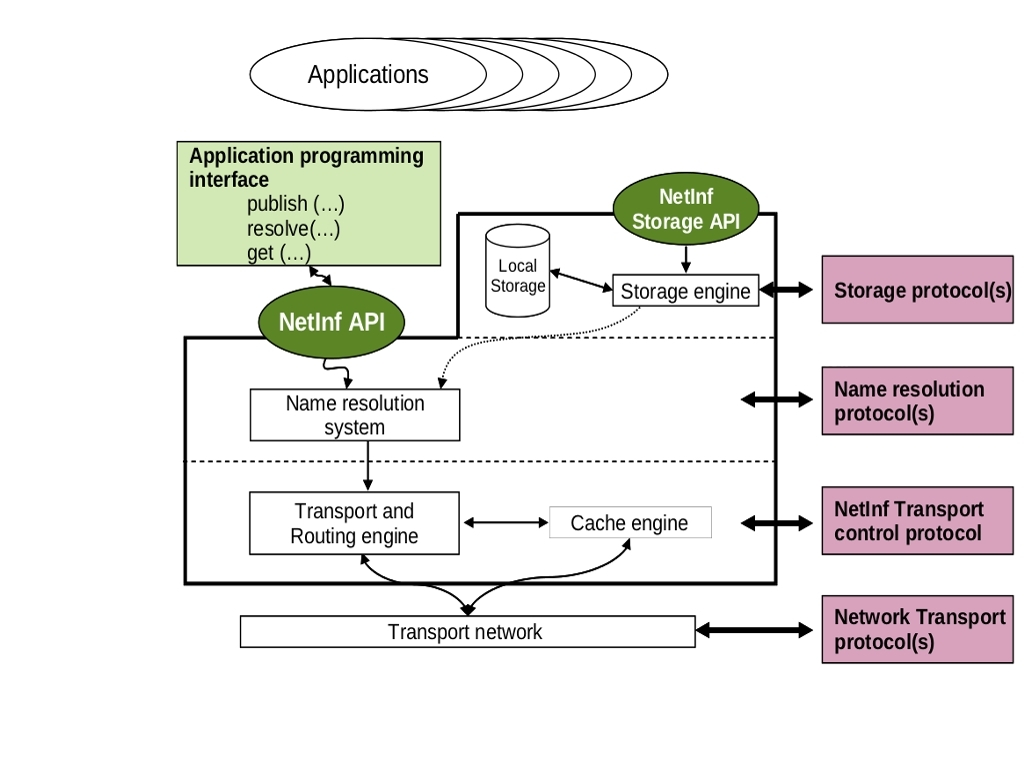
\includegraphics[height=8cm]{2.jpg}
\caption{Networking of Information Overview}
\end{center}
\end{figure}

The basic idea of Network of Information (NetInf) is to
move from today’s host centric networking paradigm to an
information centric networking paradigm where the
information objects are the primary components of
networking. One key aspect is that the information objects
are named independent of the hosts they are stored on. In NetInf,users request the information through a well-defined API by
specifying the name of an information object using the get()
primitive at the NetInf API in Figure 1.2. The name can have
cryptographic properties, e.g. a hash of the content of a file
can be part of the name. The name of the information object
can then be used to verify the authenticity of the file. How
and from where the object is retrieved is decided by the
NetInf Transport and Routing engine. This makes it possible
to react to changes in the network, both in terms of topology
and load situation, in a flexible way. Information can be
stored at arbitrary caches in the network (for short-term
optimization, cf. Caching engine in Figure 1.2) and storage
units (for long-term persistent storage, cf. Storage engine in
Figure 1.2). It can also be retrieved from NetInf hosts that have
already received the information and have stored it in their
local cache. The NetInf Name Resolution System constitutes
a flexible and scalable mechanism for handling the bindings
between the object names and location, e.g. to support host,
user and object mobility. From a cloud computing point of
view, the network of information therefore offers new
technology for dealing with the “networking resources” and
“storage” boxes in Figure 1.1.
